\documentclass{article}
\usepackage{graphicx}
\usepackage[margin=1.5cm]{geometry}
\usepackage{amsmath}

\begin{document}
\twocolumn

\title{Friday Warm Up: Unit 6: Fixed axis rotation}
\author{Prof. Jordan C. Hanson}

\maketitle

\section{Memory Bank}

\begin{itemize}
\item $\vec{s} = \vec{\theta} \times \vec{r}$ ... Geometric relationship.
\item $\vec{v} = \vec{\omega} \times \vec{r}$ ... Geometric relationship.
\item $\omega_f^2 = \omega_i^2 + 2\alpha\Delta\theta$ ... Angular kinematic equation without time, and constant $\alpha$.
\item $\vec{\tau} = \vec{r} \times \vec{F}$ ... The relationship between \textit{torque}, $\vec{\tau}$, the \textit{moment arm}, $\vec{r}$, and the \textit{force}, $\vec{F}$.
\item $\vec{\tau} = I \vec{\alpha}$ ... Newton's 2nd law, in angular form.
\item $W = \vec{\tau} \cdot \vec{\theta}$ ... Definition of work, angular form.
\end{itemize}

\section{Fixed Axis Rotation, Torque, and Kinetic Energy}

\begin{enumerate}
\item \textbf{Prove that $\tau = I\alpha$}.  (a) Start with $F = ma$, and multiply both sides by $r$.  (b) Next, substitude $a$ for $\alpha$ using $a = r\alpha$.  (c) Let $I = mr^2$, and show that $\tau = I \alpha$. \\ \vspace{2.5cm}
\item \textbf{Prove the work-energy theorem, in angular form}. (a) Start with the definition of work in angular form.  (b) Use Newton's 2nd law in angular form, to substitude $I\vec{\alpha}$ for torque. (c) Assume that $\vec{\alpha} \cdot \vec{\theta} = \alpha\theta$ because these vectors are parallel, and solve the kinematic equation without time (memory bank) for $\alpha\theta$. (d) Substitute for $\alpha\theta$ in the work equation, simplify. \\ \vspace{2.5cm}
\item Suppose the right-hand bricks in Fig. \ref{fig:1} disappear.  (a) What is the torque on the system? (b) Suppose this torque moves the balance through 10 degrees.  What is the work done? (c) What is the final kinetic energy? \\ \vspace{2.5cm}
\item The moment of inertia for a solid disk with mass $M$ and radius $R$ is $I = \frac{1}{2}MR^2$.  (a) Suppose a grindstone, used to sharpen blades, has a mass of 10 kg and a radius of 15 cm.  What is the moment of inertia in kg m$^2$? (b) Suppose we lay a chef's knife across the spinning, wet grindstone for sharpening.  The coefficient of friction is 0.2.  If we apply a normal force of 90 N, what is the force of friction? (c) What is the torque? (d) If the initial angular velocity of the grindstone is 120 rpm, but our knife brings it to a stop, what work is done on the stone? (e) How much time passes before the stone stops moving? \\ \vspace{2.5cm}
\end{enumerate}

\begin{figure}
\centering
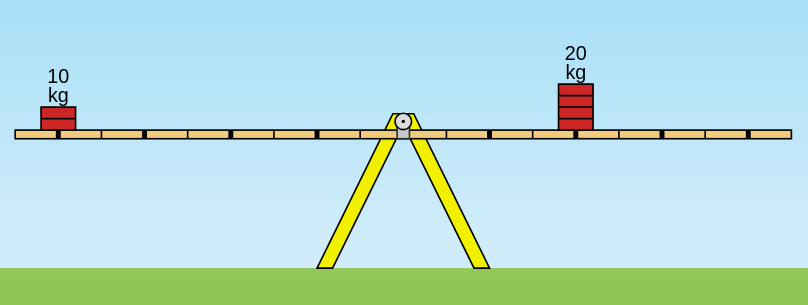
\includegraphics[width=0.4\textwidth]{figures/brick.png}
\caption{\label{fig:1} A balance between bricks of different masses.}
\end{figure}

\end{document}
